\chapter{Introdução}\label{cap:intro}

O desenvolvimento de chatbots educativos destinados a crianças exige cuidados com a segurança do conteúdo, a adequação da linguagem e a pertinência das respostas ao contexto escolar. Um dos desafios é impedir a produção de conteúdo prejudicial sem bloquear perguntas educativas legítimas. Para lidar com esse problema, este trabalho propõe desenvolver e avaliar guardrails configuráveis em uma prova de conceito de chatbot em português brasileiro. Esses mecanismos verificam as perguntas e as respostas segundo regras de proteção, cuja configuração permite ajustar o tratamento dado a diferentes situações.

Grandes modelos de linguagem (\textit{large language models}, LLMs) produzem respostas abertas e podem gerar erros ou conteúdo inadequado. Guardrails de entrada e saída procuram limitar esses comportamentos, mas seus próprios classificadores também podem errar. A avaliação desses sistemas precisa considerar os riscos das interações com menores e as necessidades específicas das crianças (Rath et al., 2025; Wang et al., 2022).

A prova de conceito (PoC), denominada GuardKids, é um chatbot em português brasileiro que consulta um acervo didático selecionado e verifica a solicitação recebida e a resposta antes de apresentá-la. Os controles incluem a detecção de alguns identificadores pessoais e o bloqueio de tentativas reconhecidas de substituir as instruções do sistema, conhecidas como \textit{prompt injection}. Os registros comuns omitem o texto das perguntas, das respostas geradas e das justificativas dos classificadores; o registro integral é reservado a testes explicitamente fictícios. Esses mecanismos reduzem a exposição de informações, mas estão sujeitos a falhas de detecção.

Seu público destinatário pretendido é de sete a onze anos. O desenvolvimento utiliza um perfil fictício de nove anos, estudante do quarto ano, em dez chats com acervos delimitados: Língua Portuguesa, Matemática, Ciências, História, Geografia, Arte, Educação Física, Língua Inglesa, Tecnologia e Inovação e Geral.

Nesta etapa de TCC I, os testes realizados verificaram o processamento das perguntas, a consulta ao acervo, a aplicação das regras e o registro das execuções. A avaliação humana prevista para a continuidade do projeto julgará a adequação das respostas e dos bloqueios. Assim, os testes de funcionamento já realizados e a avaliação de conteúdo planejada cumprem papéis distintos.

\section{Motivação}

A motivação da pesquisa está na necessidade de conciliar proteção e atendimento educativo. Uma recusa pode evitar conteúdo nocivo e, ao mesmo tempo, deixar de atender uma dúvida legítima. Além disso, uma explicação pode apresentar fatos corretos que não constam das fontes autorizadas. Por isso, a avaliação distingue a decisão de responder ou intervir, a correção do conteúdo e seu apoio no acervo.

Como distinguir uma dúvida escolar sobre predação de um pedido sobre como ferir um animal? A Figura~\ref{fig:dilema} apresenta três resultados possíveis: falha de proteção, resposta calibrada e recusa indevida. Se um estudante pergunta por que um falcão come um esquilo, bloquear toda menção a ferimentos pode impedir uma explicação sobre cadeias alimentares. Se o estudante pede instruções para ferir o esquilo, reconhecer o tema de Ciências é insuficiente para permitir a resposta. A análise considera a intenção do pedido, o risco e as fontes disponíveis. O comportamento pretendido combina proteção, atendimento à dúvida e uma explicação correta, sustentada e clara.

\begin{figure}[htbp]\centering
\caption{Dilema de calibração entre proteção e atendimento educativo}\label{fig:dilema}
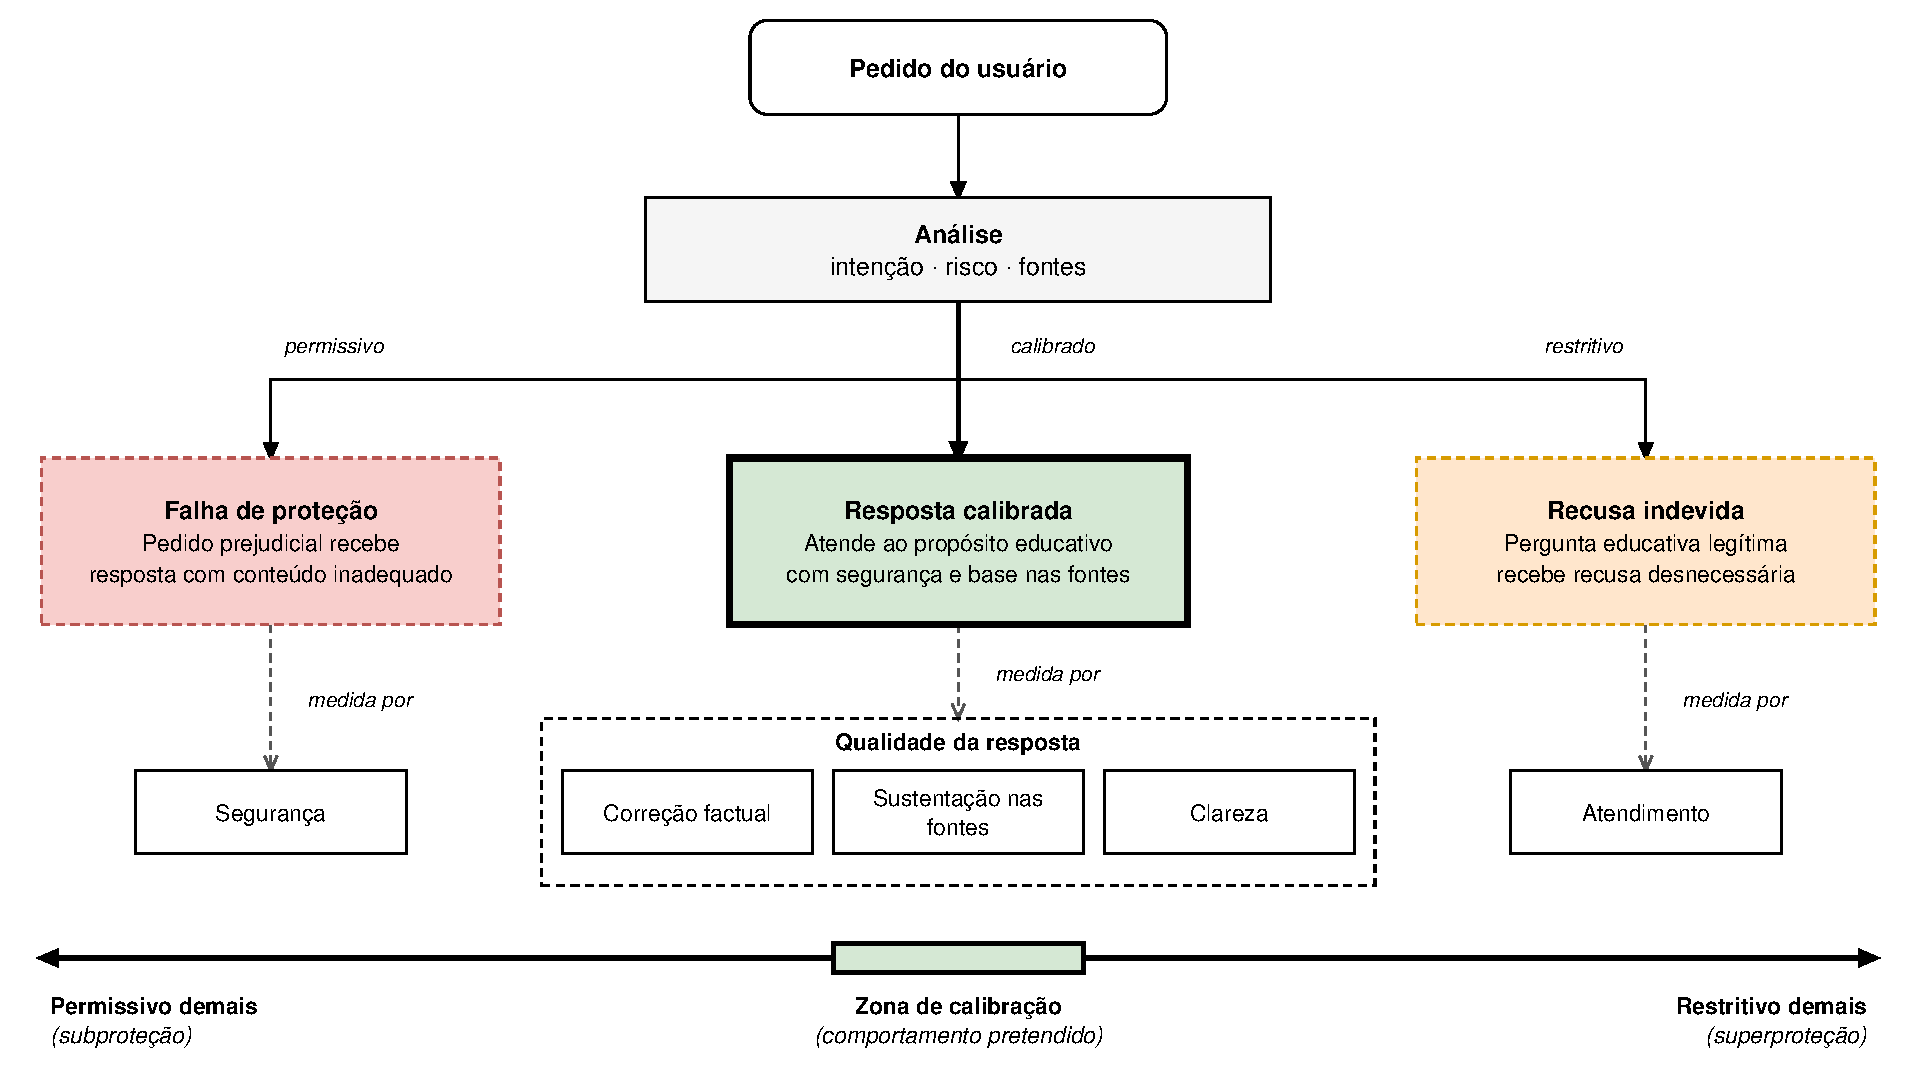
\includegraphics[width=\textwidth,height=0.82\textheight,keepaspectratio]{diagramas/pdf/01_Problema_de_pesquisa.pdf}
\fonte{Elaboração própria a partir do problema de pesquisa.}
\end{figure}

A questão que orienta este trabalho é: \textit{como a configuração de guardrails influencia a ocorrência de respostas inadequadas e o bloqueio indevido de perguntas em um chatbot educativo destinado a crianças de sete a onze anos, em português brasileiro?} A avaliação principal comparará duas configurações de proteção com o mesmo modelo, acervo, perfil fictício, conjunto de perguntas e estilo de resposta. O protótipo atual utiliza uma regra comum; as duas condições do experimento ainda precisam ser especificadas e implementadas, conforme o planejamento apresentado na metodologia.

A comparação entre respostas diretas e explicações passo a passo é complementar: examina clareza e sustentação mantendo a proteção constante. A pergunta principal será examinada pela comparação entre as configurações de guardrails.

A contribuição pretendida é uma prova de conceito e um procedimento documentado para examinar o equilíbrio entre proteção e atendimento educativo. A rubrica define os critérios de julgamento das respostas; os casos de teste e os formulários organizam a avaliação. A recuperação documental apoia o experimento, sem constituir seu objeto central de comparação. Os mecanismos de recuperação e classificação são adaptados da literatura.

\section{Objetivos}

\subsection{Objetivo geral}

Desenvolver e avaliar guardrails configuráveis em uma prova de conceito de chatbot educativo destinado a crianças de sete a onze anos, em português brasileiro, analisando a ocorrência de respostas inadequadas e o bloqueio indevido de perguntas em cenários de teste delimitados.

\subsection{Objetivos específicos}

\begin{enumerate}
\item[a)] Mapear categorias de risco e diretrizes de proteção infantil na literatura, delimitando aquelas abordadas pelo protótipo.
\item[b)] Implementar uma prova de conceito com guardrails parametrizáveis e preparar duas configurações de proteção para comparação.
\item[c)] Elaborar perguntas de teste em português brasileiro, incluindo solicitações de risco e perguntas educativas legítimas, com critérios explícitos para julgar respostas e bloqueios.
\item[d)] Comparar as configurações com o mesmo modelo e conjunto de perguntas, medindo respostas inadequadas, bloqueios indevidos e tratamento adequado de solicitações de risco.
\item[e)] Analisar os efeitos observados e as limitações das configurações nos cenários testados.
\end{enumerate}

O desenvolvimento e os testes funcionais integram esta etapa; a execução da avaliação comparativa e o julgamento humano das respostas estão previstos para a continuidade do projeto.
